\documentclass[12pt,a4paper]{article}

% --- 日本語設定 -------------------------------------------------------------
\usepackage{luatexja}
\usepackage[haranoaji]{luatexja-preset}


% --- 版面・行間 -------------------------------------------------------------
\usepackage{geometry}
\geometry{top=15mm,bottom=20mm,left=25mm,right=25mm}
\usepackage{setspace}
\onehalfspacing

% --- 数式・図表・表 ---------------------------------------------------------
\usepackage{amsmath,amssymb}
\usepackage{graphicx}
\usepackage{booktabs}

% --- ハイパーリンク ---------------------------------------------------------
\usepackage{xcolor}
\usepackage{svg}
\usepackage{hyperref}
\hypersetup{
    colorlinks=true,       % 枠線ではなく文字を着色
    linkcolor=black,      % 章タイトルなど通常リンクは黒
    urlcolor=blue,        % URL は青
    citecolor=black
}

\usepackage{listings,jvlisting}
\usepackage{enumitem}
\usepackage{multirow}
\usepackage{subcaption}
\usepackage{float}
\usepackage{indentfirst}
\usepackage{pdfpages}


\linespread{1.15}


\renewcommand{\contentsname}{目次}
\renewcommand{\listfigurename}{図目次}
\renewcommand{\listtablename}{表目次}

\renewcommand{\figurename}{図}
\renewcommand{\tablename}{表}
\renewcommand{\refname}{参考文献}



% --- 日本語表記 -------------------------------------------------------------
\makeatletter
\renewcommand{\today}{%
  \number\year 年
  \ifnum\month<10 0\fi\number\month 月
  \ifnum\day<10 0\fi\number\day 日%
}
\makeatother

\title{進捗報告}
\author{下沢\,亮太郎}
\date{\today}


\begin{document}

\maketitle

\section{先週の実施予定内容}

\begin{itemize}
  \item Gemma 4 12Bを土台に検証済みデータでSFTし，4Bと同じ評価集合で比べる
  \item 雛形外への汎化を伸ばすため，雛形を追加して学習データの種別を広げる
  \item GEPAの反省プロンプトを「一般原則を優先」に差し替えた条件を試す
  \item 問題集が簡単すぎるという指摘に対し，厳密解が出ない規模の問題を混ぜる
\end{itemize}


\section{実施した内容}

\subsection{概要}

目標は「要件を入れると最適化プログラムを書く，最適化専用の小型エージェント」で，柱はGEPAによるプロンプト最適化と，プロンプト最適化とfine-tuningを交互に回すメタ最適化（DSPyのBetterTogether）である．
今回の結果は次の四点に要約できる．

\begin{enumerate}
  \item 厳密解が出ない規模の「大規模問題」20種別を導入し，学習用・評価用にinstanceを分けた．素のGemma 4 12Bはこの評価120問を1問も解けない．
  \item 検証済みの正解コードでGemma 4 12Bを学習すると，大規模評価120問でLoRAが88問，全層学習が93問を正解した．同じデータで4Bを学習すると81問で，12Bの9割強を1/3の大きさで出せる．
  \item BetterTogether（プロンプト$\rightarrow$重み$\rightarrow$プロンプト）を1周回した．学習済みモデルは学習時の指示文に張り付いており，GEPAは2回で51案を試して1案も採用できなかった．素のモデルでは指示文が動き，大規模問題で進化させた指示文が雛形問題で+19問（345$\rightarrow$364）効いた．
  \item 学習で見ていない種別（雛形外11問）では，学習を重ねるほど正解が減る（素3$\rightarrow$学習後2$\rightarrow$自己蒸留後1）．汎化の劣化は未解決である．
\end{enumerate}


\subsection{学習データとテストデータ}

学習とテストに使った問題は，出どころの違う4つの集合に分けられる（表\ref{tab:sets}）．
どの集合も「問題文」と「instance（数値データ）」と「参照解」からなり，モデルには参照値を伏せた問題文だけを渡し，返ってきた\texttt{solve()}をinstanceで実行して検証器で採点する．

\begin{table}[H]
  \centering
  \caption{問題の集合と役割}
  \label{tab:sets}
  \small
  \begin{tabular}{p{0.13\linewidth}p{0.30\linewidth}p{0.14\linewidth}p{0.20\linewidth}p{0.11\linewidth}}
    \toprule
    集合 & 中身 & 規模 & 参照解 & 役割 \\
    \midrule
    雛形問題 & 同梱100問のうち厳密に解ける89問を雛形にし，数値を変えたinstanceを生成 & 数個〜数十個の要素 & 厳密ソルバー（CP-SAT，LP，全列挙）の最適値 & 学習・テスト \\
    大規模問題 & 新たに受け取った28問を元に，20種別ごとに同じ分布のinstanceを生成 & 数百〜数千の要素．厳密解は出ない & 既存の教師コード95本を走らせた中の最良値（最適性は未証明） & 学習・テスト \\
    大規模の元問題 & 受け取った28問そのもの（prob\_301〜330） & 同上 & 同梱の参照解 & テストのみ \\
    雛形外 & 同梱100問のうち雛形にしなかった11問 & 小規模 & 同梱の参照解 & テストのみ（汎化の測定） \\
    \bottomrule
  \end{tabular}
\end{table}

雛形問題と大規模問題は，1つの種別から乱数の種を変えて多数のinstanceを作り，学習用・検証用・テスト用に分けている（表\ref{tab:split}）．
テスト用のinstanceは学習に一度も使っていない．
ただし種別は学習と共通なので，雛形テストと大規模テストが測るのは「学習で見た種類の，新しい数値の問題を解けるか」である．
学習で見ていない種類への汎化は，雛形外11問だけが測る．

\begin{table}[H]
  \centering
  \caption{分割（instance数）}
  \label{tab:split}
  \small
  \begin{tabular}{lrrrp{0.30\linewidth}}
    \toprule
    集合 & 学習用 & 検証用 & テスト用 & 分け方 \\
    \midrule
    雛形問題（89雛形） & 3,560（各40） & 356（各4） & 445（各5） & 乱数の種を分ける \\
    大規模問題（20種別） & 600（各30） & 80（各4） & 120（各6） & 種別ごとに800を生成して分割 \\
    大規模の元問題 & --- & --- & 28 & --- \\
    雛形外 & --- & --- & 11 & --- \\
    \bottomrule
  \end{tabular}
\end{table}

学習データは「問題文$\rightarrow$正解コード」の対で，コードは必ず学習用instanceで実際に実行し，検証器で正解を確かめたものだけを使った（表\ref{tab:train}）．
正解の条件は，制約違反が0で，参照解からの差が+10\%以内であること．
モデルの出力を確かめずに学習に入れたものはない．

\begin{table}[H]
  \centering
  \caption{学習データの中身}
  \label{tab:train}
  \small
  \begin{tabular}{p{0.22\linewidth}p{0.58\linewidth}r}
    \toprule
    出典 & 作り方 & 学習対 \\
    \midrule
    雛形問題の教師コード & Fable・Qwen・Gemma・Ministralが同梱問題に書いた正解コードと手書き11本，計412本を学習用instanceで実行し，正解した対だけ残す（16,480対中15,088対） & 15,088 \\
    大規模問題のOpus 5.5の解答 & 学習用600問から種別ごとに5問，計100問をOpus 5.5に「書いて試して直す」形で解かせ，正解95問のコード（中身は21種類）を他の学習用instanceでも実行して正解したもの & 630 \\
    合計（学習に使った形） & 大規模問題の630対は件数が少ないので2回ずつ入れた．最大長16,384 tokenを超えるポートフォリオ2種別の120行は落ちた & 16,228 \\
    \bottomrule
  \end{tabular}
\end{table}

図\ref{fig:data}に，問題の集合から学習データとテストデータが作られる流れを示す．

\begin{figure}[H]
  \centering
  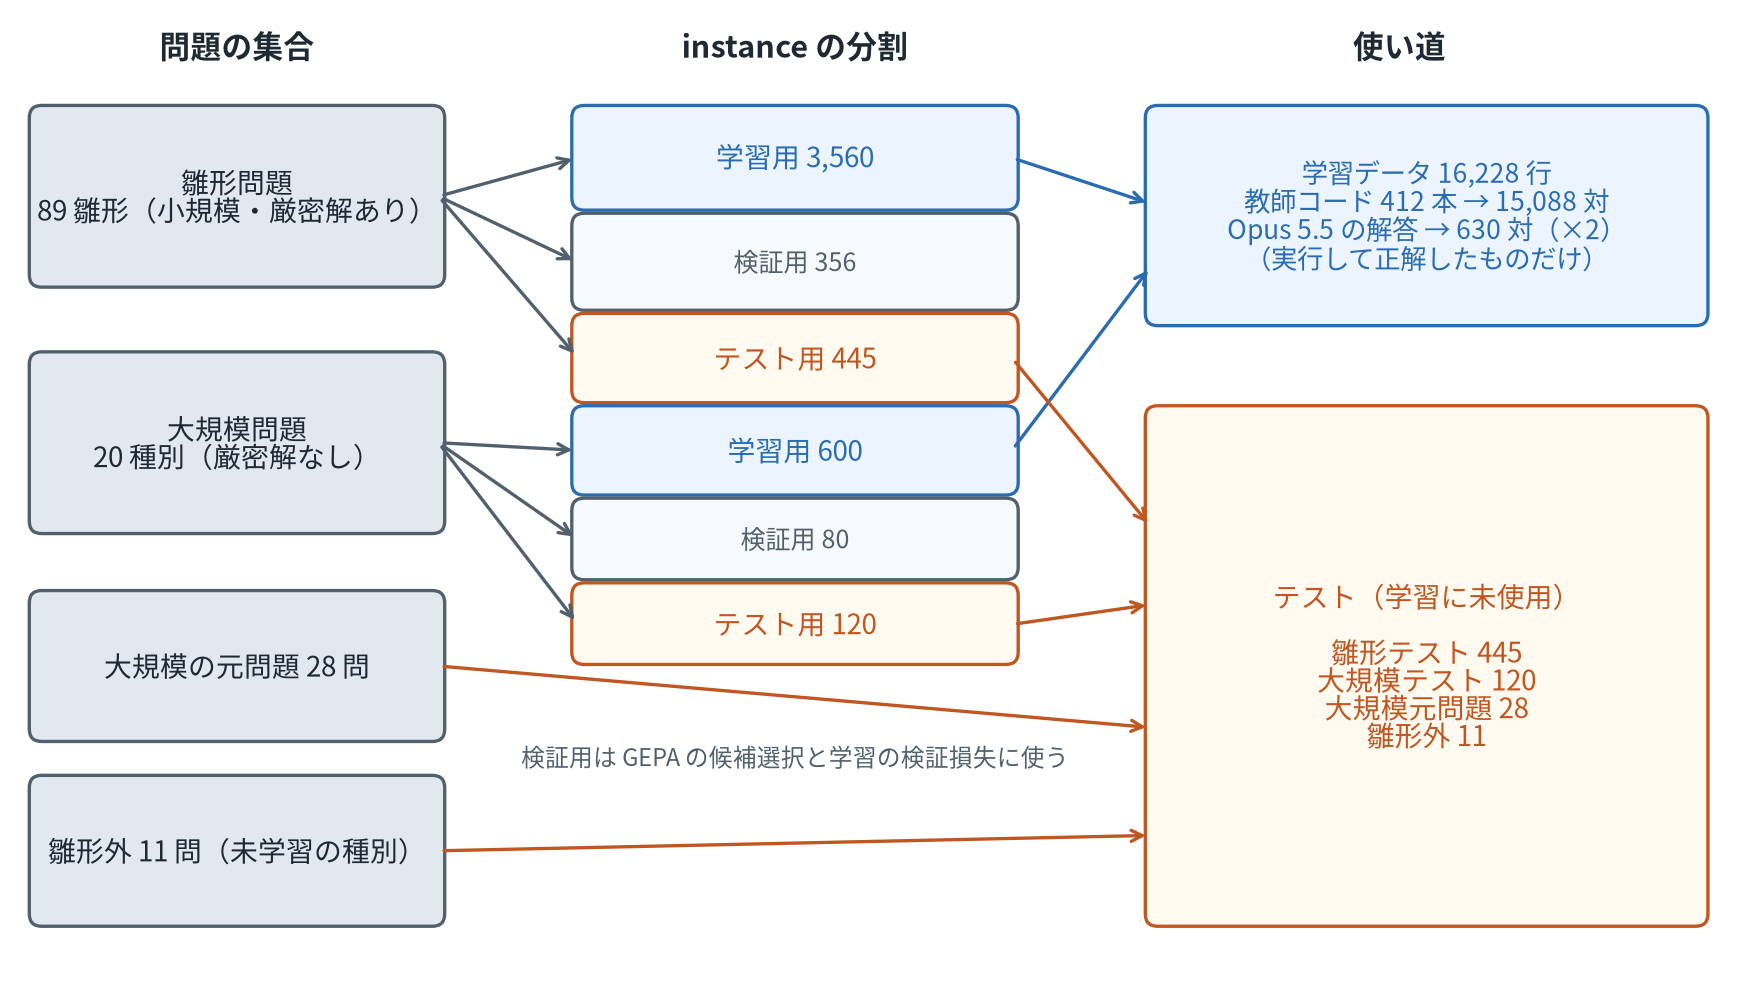
\includegraphics[width=0.95\linewidth]{./assets/data_flow.png}
  \caption{学習データとテストデータの作り方（青が学習，橙がテスト）}
  \label{fig:data}
\end{figure}

学習データに入っていない種別が大規模問題に3つある．
ポートフォリオ2種別は問題文に収益率の行列がそのまま入って4万token近くあり，学習の最大長を超えた．
乗務員ペアリングは，元問題2つで規則が違う（各便ちょうど1回か，1回以上か）のに検証器が両方に重複を許していたため，問題文どおりに解いたOpusの解が不正解と判定され，学習データが0件になった．
この3種別（テスト18問）は，学習済みモデルにとって実質的に「見ていない種別」である．


\subsection{大規模問題での特化学習と小型化}

表\ref{tab:train}の16,228行でGemma 4 12Bを学習した（表\ref{tab:result}）．
LoRAは全線形層にrank 32のadapterを足してH200 1枚で5時間38分，全層学習は120億パラメータすべてを更新してH200 2枚で6時間7分である．
同じデータでAgents-A1-4BもLoRAで学習した（3時間39分）．
いずれも1 epoch，思考を書かずに直接コードを出す形式である．

\begin{table}[H]
  \centering
  \caption{正解数（違反0・参照解から+10\%以内）}
  \label{tab:result}
  \small
  \begin{tabular}{lrrrr}
    \toprule
    モデル & 雛形テスト445 & 大規模テスト120 & 大規模元問題28 & 雛形外11 \\
    \midrule
    素のGemma 4 12B（思考なし） & 345 & 0 & 3 & 3 \\
    Qwen3.6 27B（思考あり） & --- & 4 & --- & --- \\
    Gemma 4 12B LoRA & 442 & 88 & 12 & 2 \\
    Gemma 4 12B 全層学習 & \textbf{445} & \textbf{93} & \textbf{14} & --- \\
    Agents-A1-4B LoRA & 440 & 81 & 10 & 3 \\
    \bottomrule
  \end{tabular}
\end{table}

注: 乗務員ペアリングの検証器と参照解を評価後に直したところ，素のGemma 4 12Bの大規模テストは1問が正解に変わる（0$\rightarrow$1）．他の条件の数字は変わらない．

\begin{figure}[H]
  \centering
  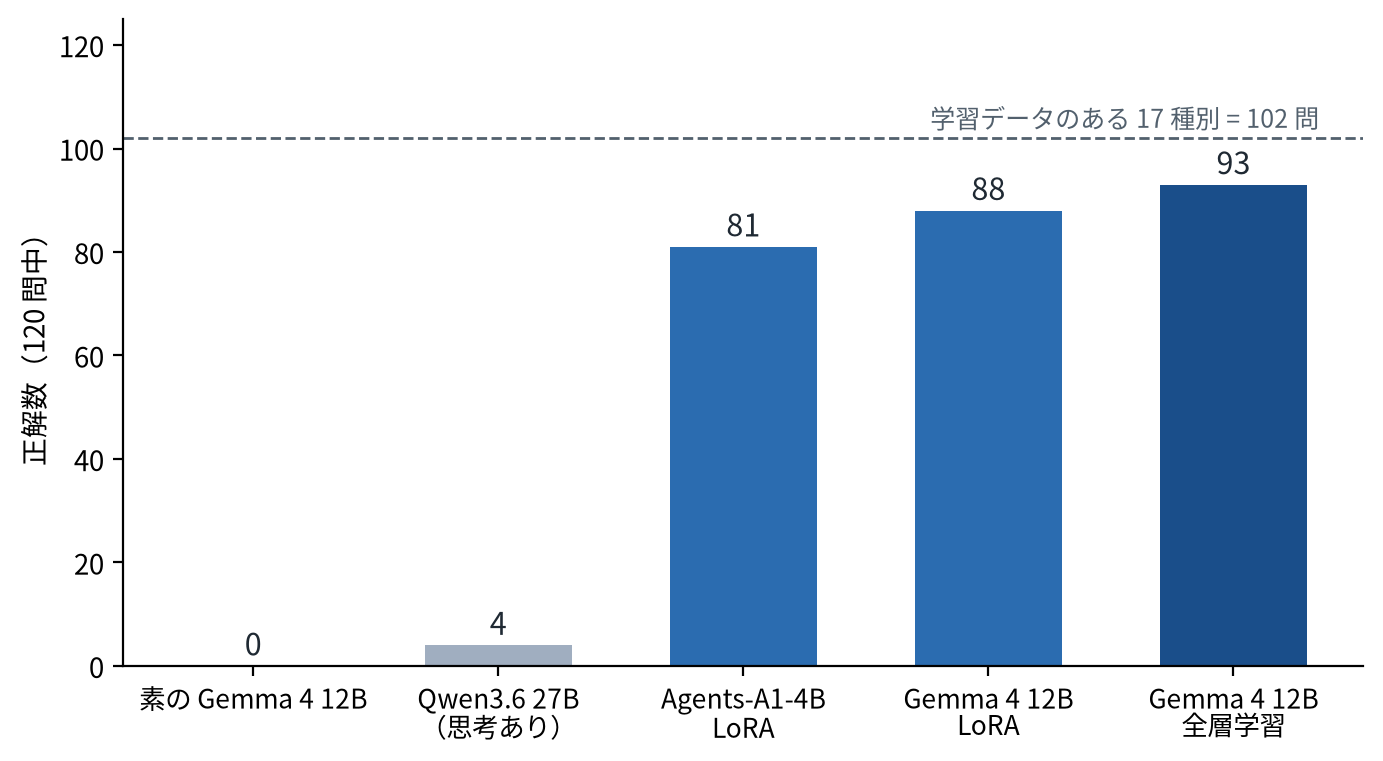
\includegraphics[width=0.85\linewidth]{./assets/hard_test_correct.png}
  \caption{大規模テスト120問の正解数（破線は学習データのある17種別の問題数）}
  \label{fig:hard}
\end{figure}

大規模テストで学習後のモデルが外した問題の大半は，学習データに入っていない3種別（18問）である（図\ref{fig:hard}）．
学習済みの17種別に限ると，全層学習は102問中93問，LoRAは88問，4Bは81問を正解した．
全層学習の正解のうち81問は，参照解（主にClaude Fableが10分かけて出した解）と同等以上だった．
LoRAと全層学習の差は問題単位で8対3（大規模テスト）で，統計的に有意ではない．

全層学習の1回目は，重みをbf16のまま更新したために失敗した（大規模テスト0問）．
学習率1e-5の更新がbf16の丸め幅より小さく，大半が消えていた．
重みをfp32で持ち，計算だけbf16で行う混合精度に直すと，検証損失が0.0305から0.0023に下がり，上記の結果になった．


\subsection{交互最適化（BetterTogether）1周目}

DSPyの\texttt{BetterTogether(p=GEPA, w=BootstrapFinetune, strategy="p -> w -> p")}と同じ順序で，上のLoRAモデル（S0）から1周回した．
プロンプト側はGEPA（反省はQwen3.8，一般則だけを書かせる反省テンプレート），重み側は「自分で解いて正解したものを足して学習し直す」である（表\ref{tab:bt}）．

\begin{table}[H]
  \centering
  \caption{1周の経過}
  \label{tab:bt}
  \small
  \begin{tabular}{p{0.13\linewidth}p{0.42\linewidth}p{0.36\linewidth}}
    \toprule
    段 & 内容 & 結果 \\
    \midrule
    p（GEPA） & S0の指示文を進化（6時間51分） & 46案を試して採用0．指示文は変わらず \\
    w（自己蒸留） & S0で大規模の学習用600問を解き，正解した452問を学習データに足して学習し直す（S1） & 雛形442$\rightarrow$445，大規模88$\rightarrow$91，雛形外2$\rightarrow$1 \\
    p（GEPA） & S1の指示文を進化（6時間29分） & 5案が全評価に進んだが，どれも元より低い．採用0 \\
    \bottomrule
  \end{tabular}
\end{table}

学習済みのモデルは学習時の指示文に張り付いていて，書き換えると出力の打ち切りや構文の崩れで壊れる．
このためプロンプト側は動かず，1周は実質「自分の正解で学び直す自己蒸留」になり，学習で見た種別を固める代わりに雛形外を削った．

論文（Soylu ら，EMNLP 2024）は素のモデルからプロンプトを先に最適化している．
同じ順で素のGemma 4 12BからGEPAを回すと，7案が全評価に進み，1案が採用された（検証平均0.260$\rightarrow$0.272）．
この指示文（大規模問題の学習用・検証用だけで進化させたもの）を素のGemmaに付けると，使っていない雛形テストで正解が345$\rightarrow$364に増えた（問題単位で49対30，符号検定$p \approx 0.04$）．
素のモデルではプロンプト最適化が効く．
この指示文をsystemにして同じ教師データで学習し直したモデル（SB1）を，既定の指示文で学習したS0と比べた（表\ref{tab:sb1}）．
学習で見た種別ではわずかに上回るが，問題単位の入れ替わりは大規模テストで6対5，元問題で2対0と小さく，有意ではない．
雛形外は2問のままだった．
素のモデルで+19問だった指示文の効果は，学習後にはほぼ消える．
学習データが同じなら，学習時の指示文の文面は結果をほとんど変えない，ということである．
SB1で2回目のGEPAを回しても（8時間16分），全評価に進んだ1案は元より低く（1.20対1.44），採用0で指示文は変わらなかった．
素のモデルから始めても，学習後のモデルではプロンプトが動かない点は同じである．

\begin{table}[H]
  \centering
  \caption{指示文を先に最適化してから学習した効果（正解数）}
  \label{tab:sb1}
  \small
  \begin{tabular}{llrrrr}
    \toprule
    モデル & 学習時の指示文 & 雛形テスト445 & 大規模テスト120 & 大規模元問題28 & 雛形外11 \\
    \midrule
    S0 & 既定 & 442 & 88（参照以上74） & 12 & 2 \\
    SB1 & GEPAで進化 & 445 & 89（参照以上78） & 14 & 2 \\
    \bottomrule
  \end{tabular}
\end{table}


\subsection{プロンプトのQwen3.6への転用}

素のGemma向けに進化させた指示文が他のモデルにも効くかを，Qwen3.6 27B（思考あり）の大規模テスト120問で測った．
既定の指示文では4問正解（平均0.092），進化させた指示文では9問正解（平均0.093）だった（表\ref{tab:qwen}）．
正解は倍以上に増えたが，問題単位では8対3で有意ではない（符号検定$p \approx 0.23$）．
平均スコアが動かないのは，指示文が長くなった分だけ思考が延び，出力枠65kを使い切ってコードを出せない問題が8から18に増えたためである．
Gemma向けに進化させた指示文はQwen3.6でも正解を増やす方向に働くが，Qwenの思考の長さとの兼ね合いがある．

\begin{table}[H]
  \centering
  \caption{Qwen3.6 27Bの大規模テスト120問}
  \label{tab:qwen}
  \small
  \begin{tabular}{lrrrr}
    \toprule
    指示文 & 正解 & 参照以上 & 平均スコア & 出力枠切れ \\
    \midrule
    既定（1,784字） & 4 & 1 & 0.092 & 8 \\
    GEPAで進化（4,152字） & 9 & 3 & 0.093 & 18 \\
    \bottomrule
  \end{tabular}
\end{table}


\subsection{教師候補: GLM-5.3-Flash}

前回の候補GLM-5.3-Flash（320B，活性18B）をllama.cppでH200 2枚とRAMに載せて試した．
生成は約14 token/秒で，大規模問題3問のうち2問は思考だけで出力枠32kを使い切り，残る1問も参照より約10\%悪かった．
1問40分かかって正解0で，学習データ集めには使わないと判断した．


\section{今週の予定}

\begin{itemize}
  \item 素のモデルから始める交互最適化の結果をまとめ，「プロンプトを先に最適化してから学習する」効果をS0と比べる
  \item 学習データに入っていない3種別を入れる（乗務員ペアリングの検証器を規則ごとに分ける，ポートフォリオの問題文から行列を外す）
  \item 汎化を測るため，種別の一部を学習から外して，外した種別で評価する実験を組む
  \item 4Bを本命の小型モデルとして，全層学習と交互最適化を4Bでも試す
\end{itemize}

\end{document}
